\section{Introduction to \maestro\ Multigrid}

\maestro\ uses multigrid to enforce the velocity constraint through
projections at the half-time (the MAC projection) and end of the time
step (the HG projection).  Two multigrid solvers are provided by
\boxlib---one for cell-centered data and one for node-centered (nodal)
data.  Both of these are used in \maestro.

\begin{figure}[t]
\centering
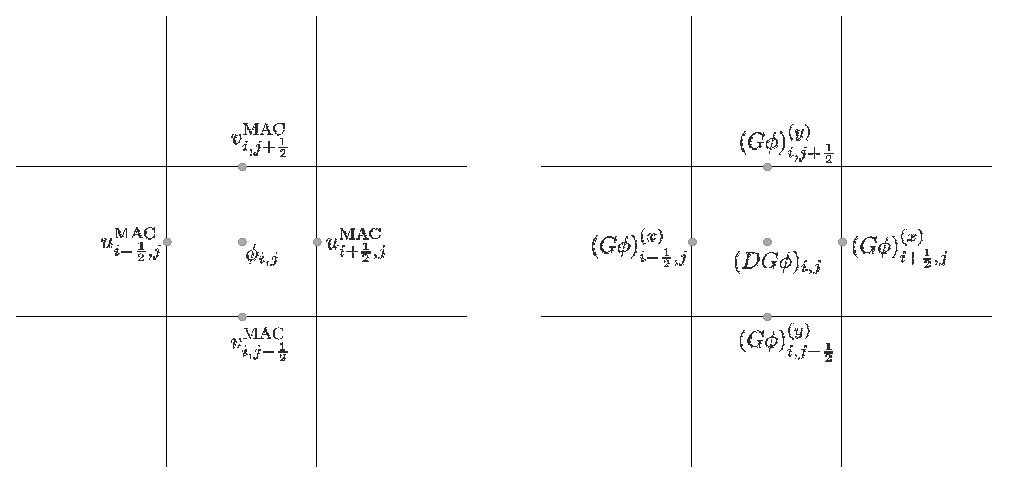
\includegraphics[width=5.5in]{\mgfigpath/MAC_mg2}
\caption{\label{fig:mg:MAC} Data centerings for the MAC projection}
\end{figure}

The MAC projection operates on the advective velocities predicted at
the cell-interfaces at the half-time.  The edge-centered velocities
are shown in Figure~\ref{fig:mg:MAC}.  If we consider purely
incompressible flow, the projection appears as:
\begin{equation}
D G \phi = D U
\end{equation}
where $D$ is the divergence operator and $G$ is the gradient operator.
In this discretization, $\phi$ is cell-centered (see
Figure~\ref{fig:mg:MAC}).  The remaining quantities are discretized as:
\begin{itemize}
\item $DU$ is cell-centered, 
  \begin{equation}
  (DU)_{i,j} = \frac{u_{i+1/2,j} - u_{i-1/2,j}}{\Delta x} + 
               \frac{v_{i,j+1/2} - v_{i,j-1/2}}{\Delta y}
  \end{equation}

\item $G\phi$ is edge-centered, on the MAC grid, as shown in
  Figure~\ref{fig:mg:MAC}.

\item $DG\phi$ is cell-centered, also shown in Figure~\ref{fig:mg:MAC},
  computed from $G\phi$ using the same differencing as $DU$.

\end{itemize}

\begin{figure}[t]
\centering
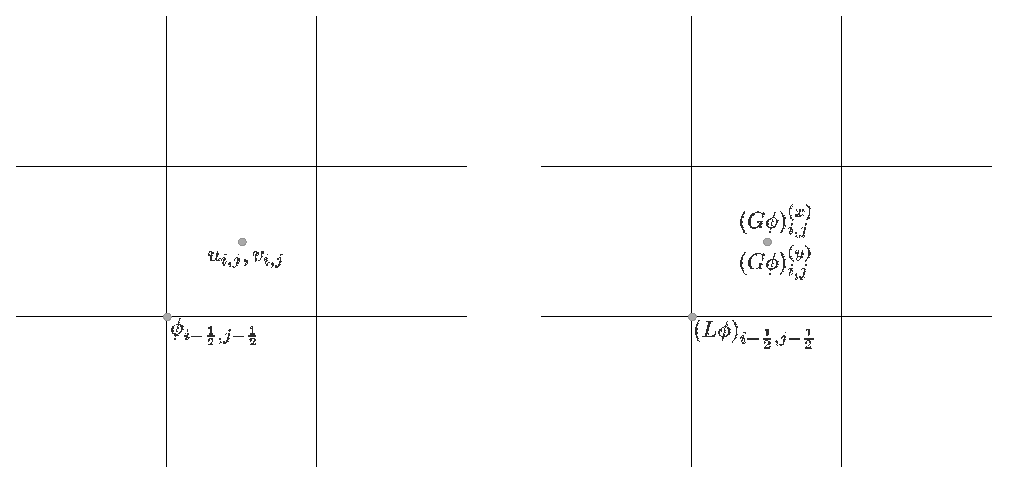
\includegraphics[width=5.5in]{\mgfigpath/HG_mg2}
\caption{\label{fig:mg:HG} Data centerings for the HG projection}
\end{figure}

The HG projection projects the cell-centered velocities at the end of
the timestep.  Here, $\phi$ is node-centered.  Figure~\ref{fig:mg:HG}
shows the locations of the various quantities involved in the HG
projection.  Again considering simple incompressible flow, we now
solve:
\begin{equation}
L \phi = D U
\end{equation}
where $L$ is a discretization of the Laplacian operator.  In this
sense, the HG projection is an {\em approximate projection}, that is,
$L \neq DG$ (in discretized form).  The various operations have the
following centerings:
\begin{itemize}

\item $DU$ is node-centered.  This is computed as:
  \begin{equation}
  (DU)_{i-1/2,j-1/2} = \frac{\frac{1}{2} (u_{i,j} + u_{i,j-1}) -
                             \frac{1}{2} (u_{i-1,j} + u_{i-1,j-1})}{\Delta x} +
                       \frac{\frac{1}{2} (v_{i,j} + v_{i-1,j}) -
                             \frac{1}{2} (v_{i,j-1} + v_{i-1,j-1})}{\Delta y} 
  \end{equation}

\item $G\phi$ is cell-centered, as shown in Figure~\ref{fig:mg:HG}.

\item $L\phi$ is node-centered.  This is a direct discretization of 
the Laplacian operator.  By default, \maestro\ uses a dense stencil
(9-points in 2-d, 27-points in 3-d).  Alternately, a {\em cross}
stencil can be used (by setting {\tt hg\_dense\_stencil = F}).  This
uses 5-points in 2-d, 7-points in 3-d.

\end{itemize}


\section{\mgtower}

The \mgtower\ is a special Fortran derived type that carries all the
information required for a \boxlib\ multigrid solve.


\section{Bottom Solvers}


\section{Convergence Criteria}


\section{Multigrid Solver Tolerances}

\label{sec:mgtol}

Beginning at the start of execution, there are several places where
either cell-centered multigrid or node-centered multigrid solves are
performed.  The outline below lists the solves one encounters, in order,
from the start of execution.  The values of the tolerances lists here
are defined in the {\tt mg\_eps} module.  To set problem-specific values
of these tolerances, place a local copy of {\tt mg\_eps.f90} in your
problem directory.

In the initialization, multigrid comes in during the initial projection
and the ``divu'' iterations.

\begin{itemize}

\item {\em initial projection} ({\tt initial\_proj} called from {\tt varden})

  The initial projection creates a first approximation to the velocity
  field by forcing the initial velocity field set by {\tt initveldata}
  to satisfy the elliptic constraint equation.  Since the initial
  velocity may be zero, there is no guarantee that a well-defined
  timestep can be computed at this point, so the source term, $S$,
  used here only involves thermal diffusion and any external heating
  term, $\Hext$---no reactions are included (see paper~III, \S 3.3).

  The initial projection can be disabled with the {\tt do\_initial\_projection}
  runtime parameter.

  The tolerances, {\tt eps\_init\_proj\_cart} and {\tt eps\_init\_proj\_sph}
  (for Cartesian and spherical respectively) are set in {\tt mg\_eps.f90}
  and have the default values of:
   \begin{center}
   \begin{tabular}{lll}
   Cartesian:   &  {\tt eps\_init\_proj\_cart} &= $10^{-12}$ \\
   spherical:   &  {\tt eps\_init\_proj\_sph}  &= $10^{-10}$
   \end{tabular}
   \end{center}


\item {\em ``divu'' iterations} ({\tt divu\_iter} called from {\tt varden})

  The ``divu'' iterations projects the velocity field from the initial
  projection to satisfy the full constraint (including reactions).
  This is an iterative process since the reactions depend on the
  timestep and the timestep depends on the velocity field (see
  paper~III, \S 3.3).  The number of iterations to take is set through
  the {\tt init\_divu\_iter} runtime parameter.

  The overall tolerance, $\epsilon_\mathrm{divu}$ depends on the iteration, $i$.
  We start with a loose tolerance and progressively get tighter.  The
  tolerances (set in {\tt divu\_iter}) are, for Cartesian:
  {\small
   \begin{center}
   \begin{tabular}{lll}
   $\epsilon_\mathrm{divu} = \left  \{ \begin{array}{lll} 
                   \min\, \{& \!\!\!\mathtt{eps\_divu\_cart} \cdot \mathtt{divu\_iter\_factor}^2 \cdot \mathtt{divu\_level\_factor}^{(\mathtt{nlevs}-1)}, \\
                            & \!\!\!\mathtt{eps\_divu\_cart} \cdot \mathtt{divu\_iter\_factor}^2 \cdot \mathtt{divu\_level\_factor}^2 \, \} & 
                           \quad \mathrm{for}~ i \le \mathtt{init\_divu\_iter} - 2 \\[2mm]
                   \min\, \{& \!\!\!\mathtt{eps\_divu\_cart} \cdot \mathtt{divu\_iter\_factor} \cdot \mathtt{divu\_level\_factor}^{(\mathtt{nlevs}-1)}, \\
                            & \!\!\!\mathtt{eps\_divu\_cart} \cdot \mathtt{divu\_iter\_factor} \cdot \mathtt{divu\_level\_factor}^2 \, \} & 
                           \quad \mathrm{for}~ i = \mathtt{init\_divu\_iter} - 1  \\[2mm]
                   \min\, \{& \!\!\!\mathtt{eps\_divu\_cart} \cdot \mathtt{divu\_level\_factor}^{(\mathtt{nlevs}-1)}, \\
                            & \!\!\!\mathtt{eps\_divu\_cart} \cdot \mathtt{divu\_level\_factor}^2 \, \} & 
                           \quad \mathrm{for}~ i = \mathtt{init\_divu\_iter}   \\
                                 \end{array}
                  \right .$ \\[10mm]
   \end{tabular}
   \end{center}
   }
   and for spherical:
   {\small 
   \begin{center}
   \begin{tabular}{ll}
   $\epsilon_\mathrm{divu} = \left  \{ \begin{array}{ll} 
                     \mathtt{eps\_divu\_sph} \cdot \mathtt{divu\_iter\_factor}^2 &
                           \quad \mathrm{for}~ i \le \mathtt{init\_divu\_iter} - 2 \, \\[2mm]
                    \mathtt{eps\_divu\_sph} \cdot \mathtt{divu\_iter\_factor}  & 
                           \quad \mathrm{for}~ i = \mathtt{init\_divu\_iter} - 1 \, \\[2mm]
                    \mathtt{eps\_divu\_sph}  &
                           \quad \mathrm{for}~ i = \mathtt{init\_divu\_iter} \, )\\
                  \end{array}
                  \right .$ \\
   \end{tabular}
   \end{center}
   }
   The various parameters are set in {\tt mg\_eps.f90} and have the default values of:
   \begin{center}
   \begin{tabular}{ll}
   {\tt eps\_divu\_cart}     &= $10^{-12}$ \\
   {\tt eps\_divu\_sph}      &= $10^{-10}$ \\
   {\tt divu\_iter\_factor}  &= 100 \\
   {\tt divu\_level\_factor} &= 10 
   \end{tabular}
   \end{center}

\end{itemize}

In the main algorithm, mulitgrid solves come in during the two MAC projections,
two (optional) thermal diffusion solves, and the final velocity projection.

\begin{itemize}

\item {\em MAC projection}  

  The MAC projection forces the edge-centered, half-time advective
  velocities to obey the elliptic constraint.  This is done both in
  the predictor and corrector portions of the main algorithm.

  There are two tolerances here.  The norm of the residual is required
  to be reduced by a relative tolerance of $\epsilon =
  \min \{ \mathtt{eps\_mac\_max}, \mathtt{eps\_mac} \cdot
  \mathtt{mac\_level\_factor}^{(\mathtt{nlevs}-1)} \}$. A separate
  tolerance is used for the bottom
  solver, $\epsilon_\mathrm{bottom} =
  \mathtt{eps\_mac\_bottom}$.  These parameters are set in {\tt
    mg\_eps.f90} and have the default values:
   \begin{center}
   \begin{tabular}{ll}
   {\tt eps\_mac}           &= $10^{-10}$ \\
   {\tt eps\_mac\_max}           &= $10^{-8}$ \\
   {\tt mac\_level\_factor} &= 10 \\
   {\tt eps\_mac\_bottom}   &= $10^{-3}$
   \end{tabular}
   \end{center}


  %an absolute tolerance of $\epsilon_\mathrm{abs} =
  %\epsilon \cdot ||U^\mathrm{ADV}||_\infty / \Delta x$

\item {\em thermal diffusion}

  This uses the same {\tt mac\_multigrid} routine as the MAC
  projection, so it uses the same tolerances.  The only difference is
  that the absolute tolerance is based on the norm of $h$ now, instead
  of $U^\mathrm{ADV}$.

\item {\em velocity projection}

  The final velocity projection uses a tolerance of $\epsilon = \min \{
  \mathtt{eps\_hg\_max}, \mathtt{eps\_hg} \cdot \mathtt{hg\_level\_factor}^{(\mathtt{nlevs} - 1)} \}$.  This tolerance
  is set in {\tt hgproject} using the parameter values specified in {\tt mg\_eps.f90}.  A separate
  tolerance is used for the bottom
  solver, $\epsilon_\mathrm{bottom} = \mathtt{eps\_hg\_bottom}$.


  The default parameter values are:
   \begin{center}
   \begin{tabular}{ll}
   {\tt eps\_hg}     &= $10^{-12}$ \\
   {\tt eps\_hg\_max}      &= $10^{-10}$ \\
   {\tt hg\_level\_factor}  &= 10 \\
   {\tt eps\_hg\_bottom}   &= $10^{-4}$
   \end{tabular}
   \end{center}

\end{itemize}

